% CVPR 2024 Paper Template; see https://github.com/cvpr-org/author-kit

\documentclass[10pt,twocolumn,letterpaper]{article}

%%%%%%%%% PAPER TYPE  - PLEASE UPDATE FOR FINAL VERSION
% \usepackage{cvpr}              % To produce the CAMERA-READY version
\usepackage[review]{cvpr}      % To produce the REVIEW version
% \usepackage[pagenumbers]{cvpr} % To force page numbers, e.g. for an arXiv version

% Import additional packages in the preamble file, before hyperref
%
% --- inline annotations
%
\usepackage[dvipsnames]{xcolor}
\newcommand{\red}[1]{{\color{red}#1}}
\newcommand{\todo}[1]{{\color{red}#1}}
\newcommand{\TODO}[1]{\textbf{\color{red}[TODO: #1]}}
% --- disable by uncommenting  
% \renewcommand{\TODO}[1]{}
% \renewcommand{\todo}[1]{#1}



% It is strongly recommended to use hyperref, especially for the review version.
% hyperref with option pagebackref eases the reviewers' job.
% Please disable hyperref *only* if you encounter grave issues, 
% e.g. with the file validation for the camera-ready version.
%
% If you comment hyperref and then uncomment it, you should delete *.aux before re-running LaTeX.
% (Or just hit 'q' on the first LaTeX run, let it finish, and you should be clear).
\definecolor{cvprblue}{rgb}{0.21,0.49,0.74}
\usepackage[pagebackref,breaklinks,colorlinks,citecolor=cvprblue]{hyperref}

%%%%%%%%% PAPER ID  - PLEASE UPDATE
\def\paperID{*****} % *** Enter the Paper ID here
\def\confName{HTCV}
\def\confYear{2024}

%%%%%%%%% TITLE - PLEASE UPDATE
\title{DOFA - Hot topics in Computer Vision}

%%%%%%%%% AUTHORS - PLEASE UPDATE
\author{Matti J. Frind\\
TU Berlin\\
{\tt\small matti@frind.de}
% For a paper whose authors are all at the same institution,
% omit the following lines up until the closing ``}''.
% Additional authors and addresses can be added with ``\and'',
% just like the second author.
% To save space, use either the email address or home page, not both
}

\begin{document}
\maketitle
\begin{abstract}
Large language models have shown impressive performance gains for various tasks in language processing in the last few years. % https://arxiv.org/abs/2402.06196
It is reasonable to think that it is possible to overcome some of the problems in remote sensing image processing, like scarcity of labeled data, with the help of foundational vision models.

In this work, we provide an evaluation of the DOFA model when used on the BigEarthNet dataset. % https://arxiv.org/abs/2407.03653
This includes an analysis of the feature vectors and different approaches for using these features for multi-label classification.

We've seen reasonable performances across different metrics but no improvement compared to other models trained on BigEarthNet. % https://ieeexplore.ieee.org/stamp/stamp.jsp?tp=&arnumber=9096309
\end{abstract}    
\section{Introduction}
\label{sec:intro}

The success of computer vision deep learning models relies heavily on the large amounts of data available for training on the internet \cite{8237359}.
In the domain of remote sensing, however, labeled data is hard to obtain because labeling is a complicated task that requires expert knowledge and there is a much wider range of sensors compared to standard RGB cameras of everyday cameras. \cite{dofa}.
There are multiple ways to address this issue, such as using synthetic data or semi-supervised learning algorithms. Following the breakthroughs of LLMs and the concept of pretraining foundation models on a wide range of tasks, recent research has attempted to transfer this concept to the area of remote sensing computer vision \cite{bommasani2022opportunitiesrisksfoundationmodels}.

This report focuses on one foundational model called 'DOFA' \cite{dofa}
and evaluates it on a new downstream task for comparison with other foundation models. The used dataset is called BigEarthNet \cite{bigearthnet}
and we will be utilizing the Sentinel-1 data. We will provide results using different metrics for the multi-label classification of both the 19-class and 43-class variants.

We will analyze the meaningfulness of the features computed by the DOFA model by applying a UMAP transformation \cite{umap-paper}. Afterward, we will use the features as input data for training various classifiers on the classification task.


\begin{figure}[h]
	\centering
	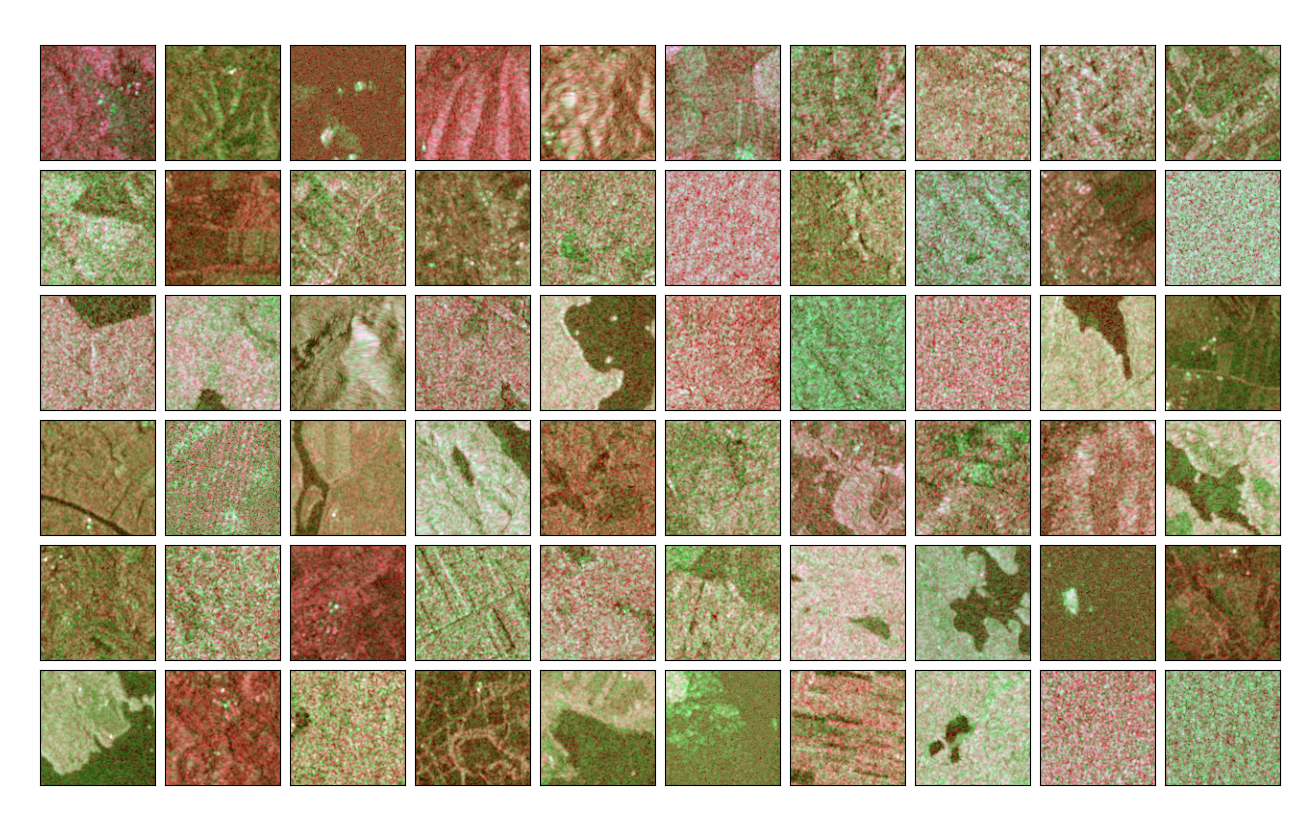
\includegraphics[width=\columnwidth]{images/example-images.png}
	\caption{False color visualization of some images from Sentinel-I satellites as part of the BigEarthNet dataset \cite{bigearthnet}}
	\label{fig:example-image}
\end{figure}
\section{Related research}
\label{sec:related}

%CHECK THE FOLLOWING:
%- Find a logical structure of related work.
%- Avoid buzzword dropping.
%- Briefly summarize related works.
%→ Make sure its understandable.
%- Put your work into context
%→ What are similarities / differences.
%- No need to be exhaustive.
%→ Focus on main papers.


Self-supervised learning has been used for several years to accomplish different tasks in remote sensing and is also applicable for training larger multi-modal foundational models \cite{dofa, satmae, croma}.
There are two primary methods to generate meaningful features. The first method is to use contrastive learning \cite{chen2020simpleframeworkcontrastivelearning}, where two views of the same image should be close together in feature space, while two views of different images should be far apart from each other. These two views can be simple image transformations or, for example, the same area of the earth captured by a different sensor.
There are many examples with different strategies for this contrastive learning approach \cite{satmae, ayush2022geographyawareselfsupervisedlearning}.
Research has shown that this approach tends to produce models that ignore information in the data that is not shared between the augmented views, regardless of whether this information would be useful in later downstream tasks \cite{tian2020makesgoodviewscontrastive}.
Because of this, it is crucial to select an appropriate augmentation strategy as this decision heavily affects the performance of the model \cite{neumann2019indomainrepresentationlearningremote}.

The alternative to contrastive learning is learning to reconstruct images. An example of this approach is SimMIM \cite{xie2022simmimsimpleframeworkmasked}.
These models can be easily scaled as they don’t rely on image pairs \cite{he2021maskedautoencodersscalablevision},
but they require additional fine-tuning to become useful for downstream tasks \cite{lehner2023contrastivetuninglittlehelp}.

Most previous foundational models were trained on a single sensor type. For example, Scale-MAE \cite{scalemae} is for optical data, SatMAE \cite{satmae} for Sentinel-2 data, and so on. Although these models can be used for various downstream tasks in their specific sensor domain, they can't generalize across these domains. According to DOFA, this leads to several limitations. Models are unable to utilize most of the unlabeled data during training because it is from a different sensor type. They also lack universality when the downstream task differs from the original data as needed channels and bandwidths change based on the used sensor. Overcoming these limitations and leveraging data from various sensors is the main goal of DOFA \cite{dofa}.

Various studies have attempted to address the issue of multi-modality, such as \cite{croma, tseng2024lightweightpretrainedtransformersremote, hackstein2024exploringmaskedautoencoderssensoragnostic}.


\section{DOFA Model}
\label{sec:dofa}

\begin{figure}[h]
	\centering
	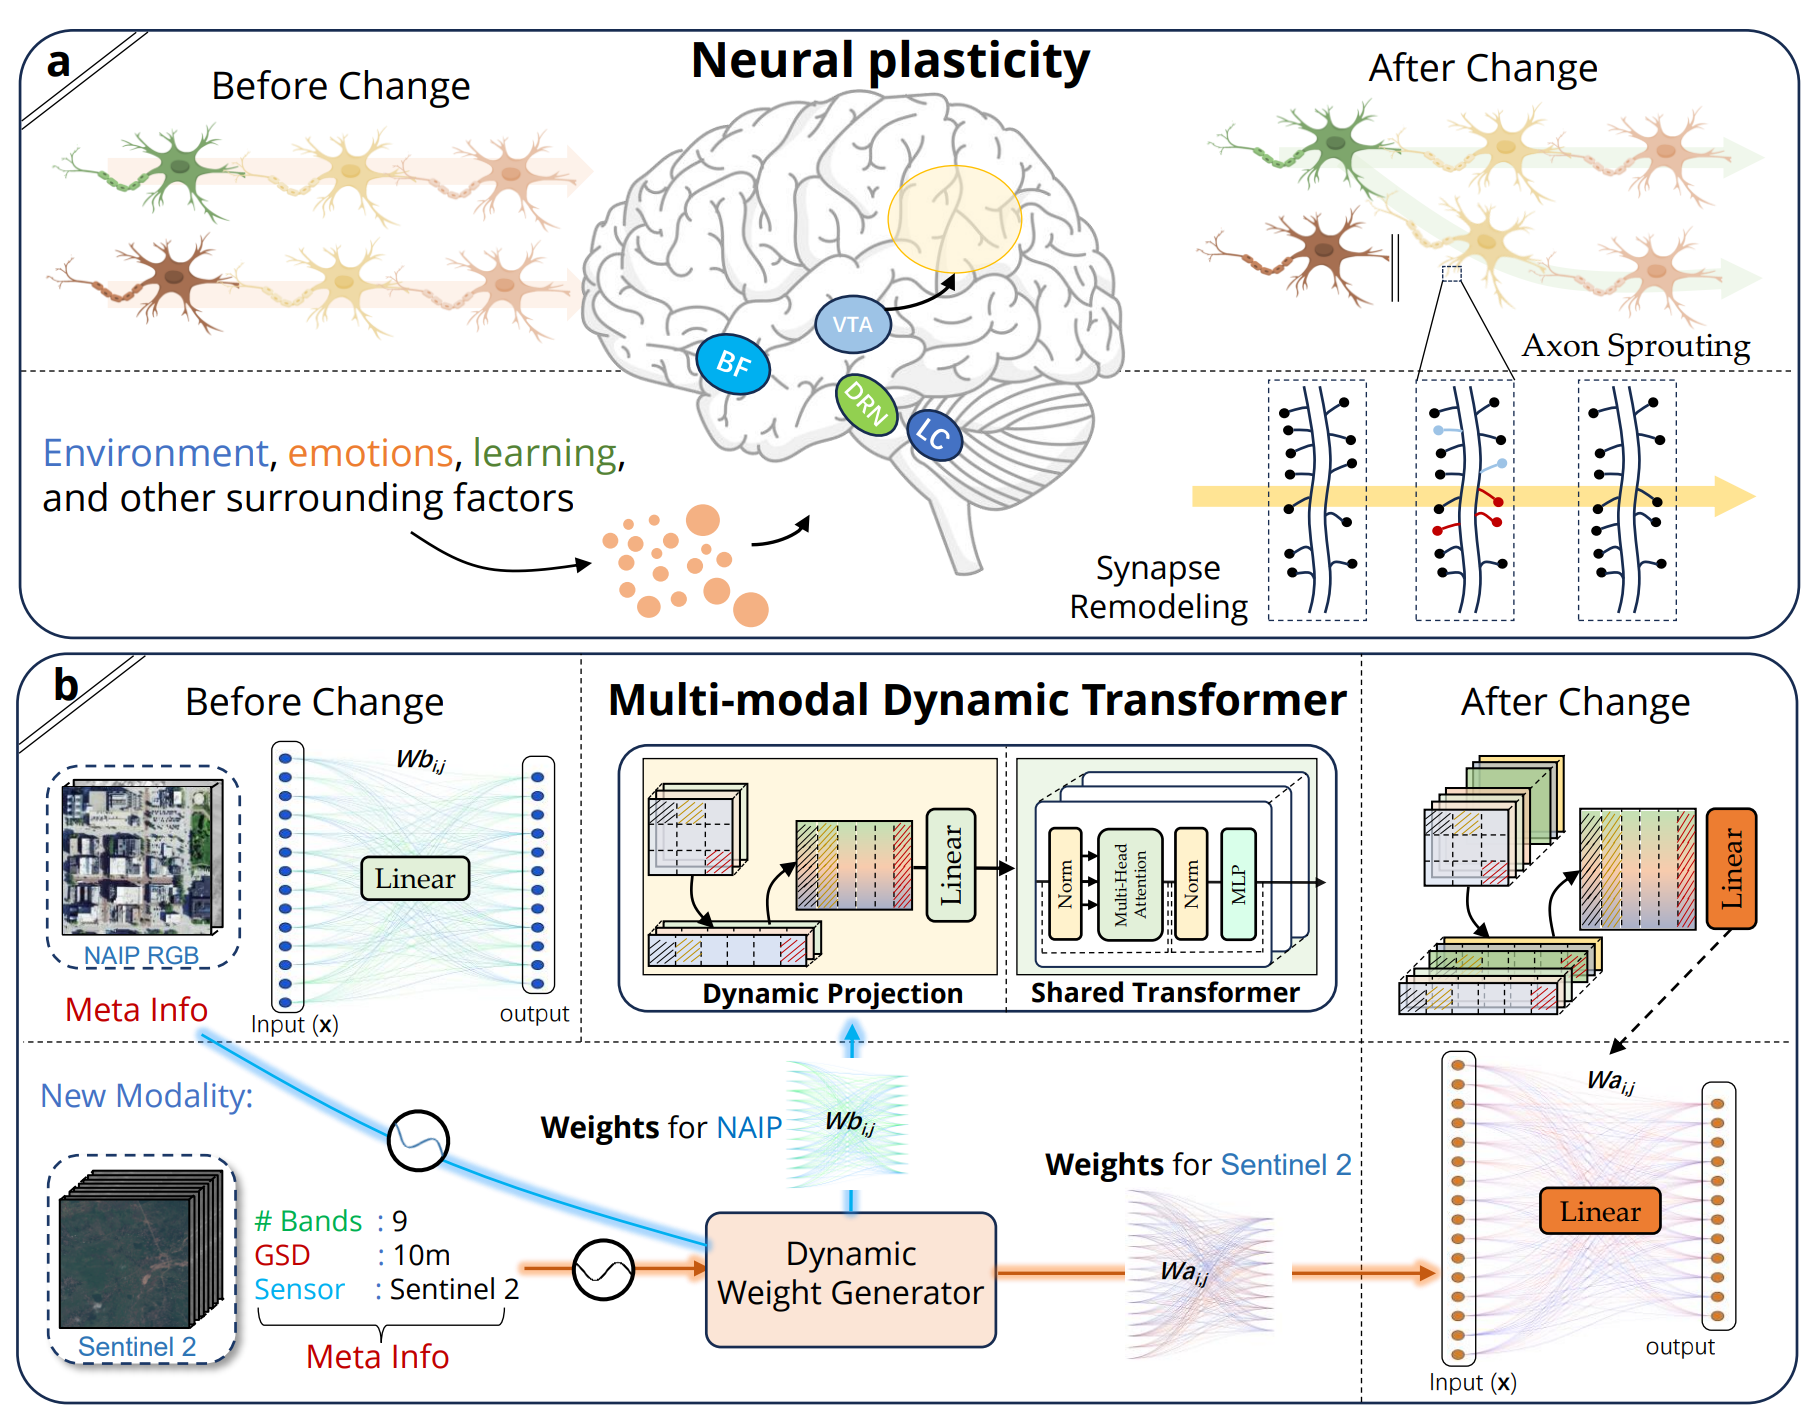
\includegraphics[width=\columnwidth]{images/dofa-concept.png}
	\caption{Visualization from the original paper \cite{dofa}. Shows the inspiration for neural plasticity from the human brain and it's application for the DOFA architecture.}
	\label{fig:dofa-concept}
\end{figure}

'DOFA' stands for \emph{'Dynamic-One-For-All'} model, inspired by the concept of neural plasticity from brain science. The main goal is to integrate various data modalities into a single framework, adaptively adjusting to different sensor inputs without needing separate models for each sensor type. This means that the model adjusts weights based on the varying wavelengths of the input data. The training process resembles that of a single large transformer model.

The authors used data from \emph{different sources and sensors} including Landsat, Sentinels, MODIS, EnMAP, Gaofen, and NAIP, which are representative of a large range of spectral bands, resolutions, and imaging types. DOFA is trained using masked images and predicting the missing patches to learn meaningful representations on unlabeled data. It uses \emph{pre-trained models} that were trained on ImageNet to enhance training efficiency and reduce training times. Additionally, as a new distillation loss is introduced to improve model performance.

The \emph{distillation loss} is derived from the concept of knowledge distillation, where we want to transfer knowledge from a larger model (e.g., trained on ImageNet), which we call the 'teacher' model to a smaller model which we call the 'student' model. The basic idea is that the student model (DOFA) is trained so that its output aligns closer to that of the teacher model. This is especially useful when it comes to data that the teacher model has already seen, which in this case refers to RGB images (for example on landscape images which are somewhat similar to remote sensing data). This setup should accelerate training convergence and enhance the overall performance. This loss is combined with the loss for image reconstruction. Together they guide the model to not only reproduce the input data correctly but also form representations that are informed by the teacher model.

The core idea of adjusting weights is through a second \emph{hypernetwork}. This secondary neural network is trained to generate weights and biases for the main network (transformer-based) to execute, based on the input data.The characteristics utilized include central wavelengths associated with each input band and their standard deviations. The hypernetwork learns during training to generate effective weights as it receives feedback on the performance of the primary network. This approach makes it possible to use tailored transformations for different modalities \emph{and} train everything in one go. The whole architecture is shown in Figure \ref{fig:dofa-concept}.

The authors claim that this approach using one foundational model \emph{reduces the computational overhead} and complexity compared to multiple specialized models. Through its multimodal training, the model should be able to handle EO tasks and data types that it hasn't seen before. This concept of multi-modality is expected to be transferable to other fields like medical image analysis and robotics.

The results in their paper show high performances in different datasets and downstream tasks compared to other approaches. The only dataset in their evaluation that is behind other approaches is the BigEarthNet for which we will provide more results.

\cite{dofa}
\section{Methodology}
\label{sec:methodology}

The images of the BigEarthNet are being fed through the DOFA model and the feature vectors are used for further analysis like UMAP visualization and training data for downstream tasks. The approach relies on PyTorch (DOFA execution, classifier training), scikit-learn (classifier training, metrics), and a Python implementation of the UMAP visualization //https://umap-learn.readthedocs.io/en/latest/index.html
\section{Experiments}
\label{sec:experiments}

\subsection{Data}

We're using the *BigEarthNet dataset* % source BigEarthNet
for our evaluations. The goal is to use the model as a feature generator and use these features for solving the multi-label classification problem with 19 classes from BigEarthNet. This dataset contains around 550.000 image patches from Sentinel-I and Sentinel-II with multi-class labels for every image. We are going to use the *Sentinel-I* images for our experiments.


The data is split into train and test set based on the implementation from the torchgeo repository. %https://torchgeo.readthedocs.io/en/latest/api/datasets.html#bigearthnet
The train dataset contains around 270.000 and the test dataset has 125.000 images.

There are high differences in the occurrence of certain classes in the dataset (see \ref{fig:class-distribution}). There are, for example, only a few images with wetlands, beaches, and moors. The metrics during the evaluation have to account for this.

\begin{figure}
  \centering
  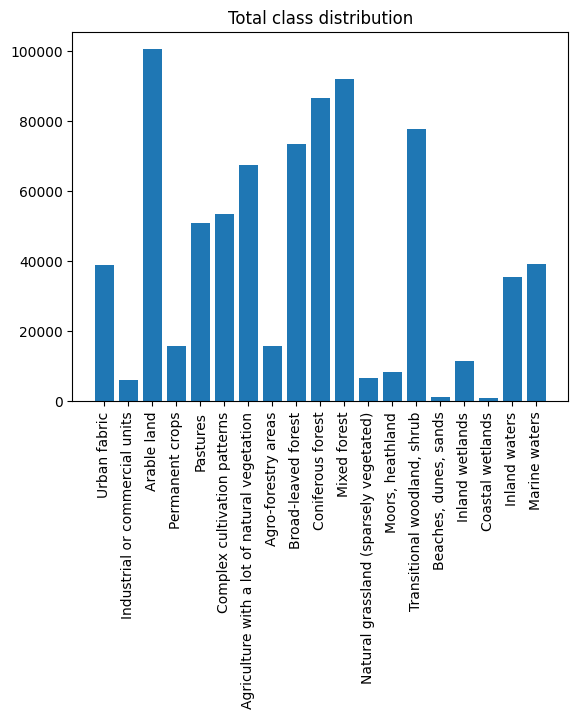
\includegraphics[width=\linewidth]{images/class_distribution.png}
  \caption{Distribution of the classes in the train dataset. This is a multiclass dataset so one can have multiple classes.}
  \label{fig:class-distribution}
\end{figure}

\begin{figure}
  \centering
  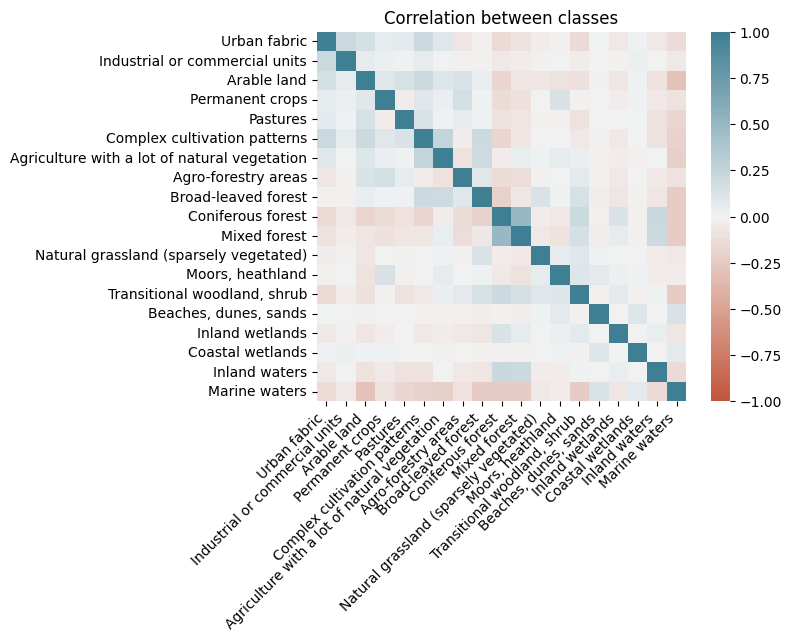
\includegraphics[width=\linewidth]{images/correlation.png}
  \caption{Correlation of classes in the train dataset}
  \label{fig:correlation}
\end{figure}

We analyzed the correlation between classes of BigEarthNet and the results are displayed in \ref{fig:correlation}. The classes are mostly uncorrelated with some exceptions like the high likeliness that coniferous forests are usually also mixed forests and marine waters are mostly not in the same images as all the other vegetation forms.

\subsection{Performance Metrics}

We decided to compute multiple metrics for evaluating the performance of the models in the classification tasks. We provide results for *f2-micro, f2-macro* (see XXXX for implementation) % https://scikit-learn.org/stable/modules/generated/sklearn.metrics.fbeta_score.html
*, hamming-loss*, and *precision * scores (see XXXX for implementation) % https://scikit-learn.org/stable/modules/generated/sklearn.metrics.precision_score.html
. We also calculate precision and f1 scores for individual classes.

\subsection{Results}

First, we calculated feature vectors using DOFA for all the images in BigEarthNet (Sentinel-I) and saved them for further use. All the following analyses use these vectors for visualizations or the downstream classification task.

\subsubsection{UMAP Feature analysis}

\begin{figure}
  \centering
  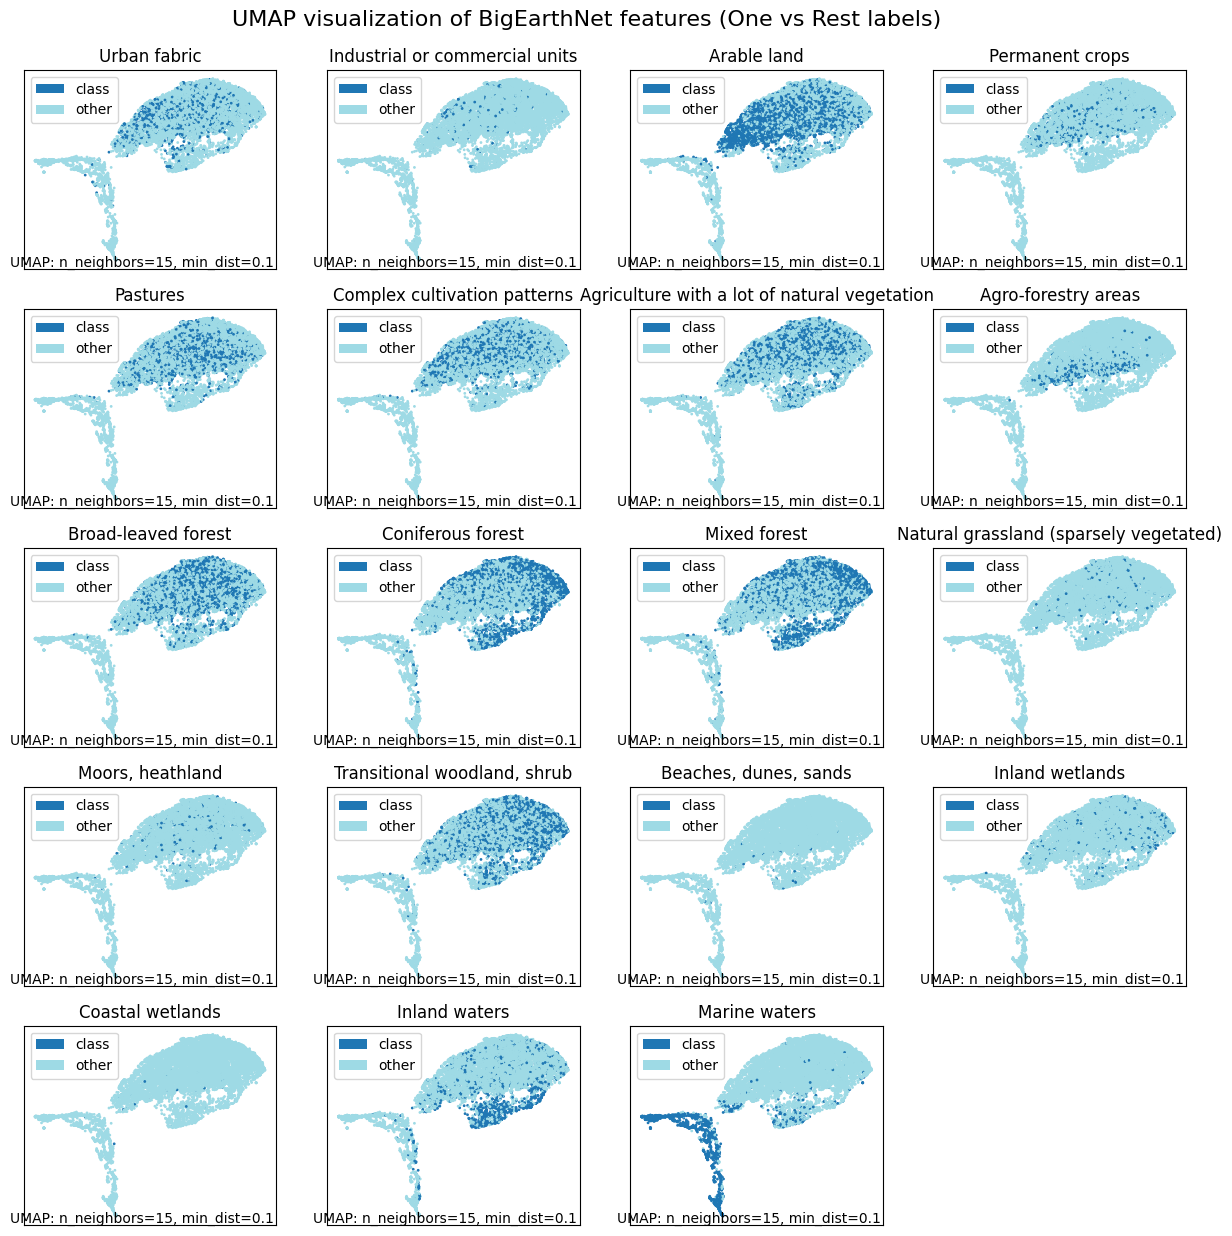
\includegraphics[width=\linewidth]{images/umap.png}
  \caption{Visualization of the 19 classes in a UMAP transformed space (one vs. rest)}
  \label{fig:umap}
\end{figure}

In \ref{fig:umap} are the occurrences of different classes in a UMAP transformed 2D space visualized. Because one image has multiple labels we choose the visualization via multiple charts. In this visualization, we expect different classes to be in different data cloud regions. As we can see this holds for a lot of the classes. Most notably we have a separate region for all marine water images (right bottom chart). As we've seen in @correlation this class is negatively correlated with most of the other classes so a separation in this visualization is plausible.
It appears that arable land is more on the left side of the main region while forests, woodlands, etc. are more on the right side.

With the results of this visualization, we expect that the feature vectors of DOFA capture the semantic meaning of the different images and it should be possible to train a classifier on top of that data.

\subsubsection{Classification}

We used the feature vectors of DOFA to train different ML algorithms for the given classification task. All the approaches use the same data split. In @test-results are the final results of these experiments.

\begin{figure}
  \centering
  \begin{tabular}{||c c c c c||} 
    \hline
    sdsd & $F^2_{macro}$ \% & $F^2_{micro}$ \% & hamming loss & $P_{macro}$ \%  & $P_{micro}$ \% \\ [0.5ex] 
    \hline\hline
    Test & 1 & 6 & 87837 & 787 & 787 \\ 
    \hline
    Test & 2 & 7 & 78 & 5415 & 787 \\
    \hline
    Test & 3 & 545 & 778 & 7507 & 787 \\
    \hline
    Test & 4 & 545 & 18744 & 7560 & 787 \\
    \hline
    Test & 5 & 88 & 788 & 6344 & 787 \\ [1ex] 
    \hline
  \end{tabular}
  \caption{Test results of different classification approaches on the 19-class multi-label classification task \footnote{Some classes contain so few examples that they are not in the test dataset and receive a $F^2$ score of 0.}}
  \label{fig:test-results}
\end{figure}

#figure(
  table(
    columns: (auto, auto, auto, auto, auto, auto),
    inset: 3pt,
    align: horizon,
    table.header(
      [], [$F^2_"macro"$ (%)], [$F^2_"micro"$ (%)], [*hamming loss*], [$P_"macro"$ (%)], [$P_"micro"$ (%)], 
    ),
    "Random Forest",
    $21.4$,
    $35.8$,
    $0.123$,
    $52$,
    $bold(72)$,
    "Linear Probing",
    $22.9$,
    $35.3$,
    $0.124$,
    $49$,
    $70$,
    "MLP",
    $bold(34.5)$,
    $bold(47.8)$,
    $bold(0.113)$,
    $bold(58)$,
    $71$,
  ),
  caption: "Test results of different classification approaches on the 19-class multi-label classification task" + footnote("Some classes contain so few examples that they are not in the test dataset and receive a " + $F^2$ + " score of 0.")
) <test-results>

#figure(
  table(
    columns: (auto, auto, auto, auto, auto, auto),
    inset: 3pt,
    align: horizon,
    table.header(
      [], [$F^2_"macro"$ (%)], [$F^2_"micro"$ (%)], [*hamming loss*], [$P_"macro"$ (%)], [$P_"micro"$ (%)], 
    ),
    "Random Forest",
    $9.46$,
    $33.7$,
    $0.056$,
    $24$,
    $71$,
    "Linear Probing", // todo the rest of the lines
    $22.9$,
    $35.3$,
    $0.124$,
    $49$,
    $70$,
    "MLP",
    $bold(34.5)$,
    $bold(47.8)$,
    $bold(0.113)$,
    $bold(58)$,
    $71$,
  ),
  caption: "Test results of different classification approaches on the 43-class multi-label classification task"
) <test-results-43>

There are notable differences in the performance of the chosen approaches. MLP has the best performance over most of the metrics. However random forest classifier and linear probing also have similar scores in $P_"micro"$ and $P_"macro"$. All classifiers have significant differences between their micro and macro averaged scores. When we compare the $F^2$ scores per class we can see the cause for these values (@scores-by-class). There is a high variance in the performance across classes which reaches from $0%$ $F^2$ score to about $90%$ $F^2$ score. This leads to the different averaging variants resulting in different scores. We can also see that MLP manages to achieve higher scores than the linear classifier over more classes.

#figure(
  grid(
    columns: (auto, auto),
    rows: (auto),
    gutter: 3pt,
    image("images/Linear Probing - f2 scores.png"),
    image("images/MLP - f2 scores.png"),
  ),
  caption: $F^2$ + " scores for every class. Left side for the linear classifier, right side for the MLP classifier."
) <scores-by-class>

This leads to the conclusion that the features generated by the DOFA model are not well linearly separable across all classes and only some achieve a $F^2$ score of over $50%$.

Random forest classifiers can separate high dimensional data, but in this case, their scores are on the same level as the linear classifier. // WHY????

#figure(
  image("images/MLP - confusion matrix.png"),
  caption: "Confusion matrices of the MLP classifier on the test set. The matrices are calculated separately for each class."
)

// REMARKS ABOUT CONFUSION MATRIX
\section{Conclusion}
\label{sec:conclusion}

%CHECK FOR THE FOLLOWING:
%- Summarize main contributions.
%- Summarize main findings.
%- What is the take home message?
%- What are possible future directions

As we have seen, the DOFA model can be used to analyze the Sentinel-1 from the BigEarthNet dataset. The features from the model contain the semantic information necessary to train a classifier to predict the related class labels. However, the model struggles to provide high-quality features for classes with low availability, which leads to mediocre classification performance and doesn't keep up to the state-of-the-art.
{
    \small
    \bibliographystyle{ieeenat_fullname}
    \bibliography{main}
}

% WARNING: do not forget to delete the supplementary pages from your submission 
% \clearpage
\setcounter{page}{1}
\maketitlesupplementary


\section{Rationale}
\label{sec:rationale}
% 
Having the supplementary compiled together with the main paper means that:
% 
\begin{itemize}
\item The supplementary can back-reference sections of the main paper, for example, we can refer to \cref{sec:intro};
\item The main paper can forward reference sub-sections within the supplementary explicitly (e.g. referring to a particular experiment); 
\item When submitted to arXiv, the supplementary will already included at the end of the paper.
\end{itemize}
% 
To split the supplementary pages from the main paper, you can use \href{https://support.apple.com/en-ca/guide/preview/prvw11793/mac#:~:text=Delete%20a%20page%20from%20a,or%20choose%20Edit%20%3E%20Delete).}{Preview (on macOS)}, \href{https://www.adobe.com/acrobat/how-to/delete-pages-from-pdf.html#:~:text=Choose%20%E2%80%9CTools%E2%80%9D%20%3E%20%E2%80%9COrganize,or%20pages%20from%20the%20file.}{Adobe Acrobat} (on all OSs), as well as \href{https://superuser.com/questions/517986/is-it-possible-to-delete-some-pages-of-a-pdf-document}{command line tools}.

\end{document}
